

\section{Hyperparameters}
\label{appendix:hps}


\begin{table}[h]
    \begin{center}
        \begin{tabular}{l c }
        \toprule
        Hyperparameter & Value \\
        \midrule
        weight decay & 0.1 \\
        grad clip norm & 1.0 \\
        LR schedule & cosine \\
        Adam $\beta_1$ & 0.9 \\
        Adam $\beta_2$ & 0.95 \\
        Context length & 2048 \\
        Batch size (tokens) & 524288 \\
        Warmup Steps & $\max(1000, 0.01 \times \textrm{train iters})$ \\
        Min LR & $0.1 \times$ Max LR \\
        \bottomrule
        \end{tabular}
    \end{center}
    \caption{Hyperparameters. These follow \cite{brown2020language}. Hyperparameters not listed here follow defaults in the Megatron codebase \cite{shoeybi2019megatron}.}
    \label{table:hps_appendix}
\end{table}

\begin{table}[h]
    \vspace{-0.3cm}
    \begin{center}
        \begin{tabular}{l c c c c c c c}
        \toprule
        Model Name & params & layers & $d_{\mathrm{model}}$ & heads & Base LR \\
        \midrule
Tiny & 50M & 8 & 512 & 8 &  $8 \times 10^{-4}$ \\  
Small & 125M & 12 & 768 & 12 &  $6 \times 10^{-4}$ \\                         
Medium & 350M & 24 & 1024 & 16 & $3 \times 10^{-4}$ \\                        
Large & 760M & 24 & 1536 & 16 &  $2.5 \times 10^{-4}$ \\                       
1.3B & 1.3B & 24 & 2048 & 16 &  $2 \times 10^{-4}$ \\                            
2.7B   & 2.7B & 32 & 2560 & 32 & $1.6 \times 10^{-4}$ \\                       
6.7B   & 6.7B & 32 & 4096 & 32  & $1.2 \times 10^{-4}$ \\                  
        \bottomrule
        \end{tabular}
    \end{center}
    \vspace{-0.3cm}
    \caption{Model architectures and base LRs we consider. These follow GPT-3 \cite{brown2020language}.}
    \label{table:param}
\end{table}



\FloatBarrier
\newpage
\section{Additional Experimental Data}
\label{appendix:experimental_data}


\begin{table}[h]
\begin{center}
\begin{tabular}{lll}
\toprule
Model size & $R^2$  & $\beta$   \\
\midrule
2.7b    & 0.9973 &  0.4184 \\
1.3b  & 0.9898 &  0.3171  \\
760m  & 0.9763 &  0.3155  \\
350m  & 0.9607 &  0.3799  \\
125m  & 0.9895 &  0.6531  \\
50m   & 0.9977 &  0.7029  \\
\bottomrule
\end{tabular}
\end{center}
\caption{The $R^2$ values and found $\beta$s of the fits in \Cref{fig:4fits}. The $R^2$s are relatively close to 1, indicating a good fit. The $\beta$s are relatively similar for models $\ge$ 350m, but are larger for the smallest models.}
\label{table:r2_scaling}
\end{table}


\begin{table}[h]
\begin{center}
\begin{tabular}{ll}
\toprule
Token Horizon & $R^2$     \\
\midrule
25B   &  1- \scinot{6.68}{-4}  \\
50B & 1 - \scinot{7.59}{-4} \\
100B  & 1 - \scinot{4.68}{-3} \\
200B  & 1 -  \scinot{2.85}{-3}  \\
400B  & 1 -  \scinot{1.76}{-3} \\
\bottomrule
\end{tabular}
\end{center}
\caption{The $R^2$ values of the fits in \Cref{fig:350m_curves}. They are very close to 1, indicating a great fit.}
\label{table:r2_each}
\end{table}







\begin{figure}[h]
\begin{center}
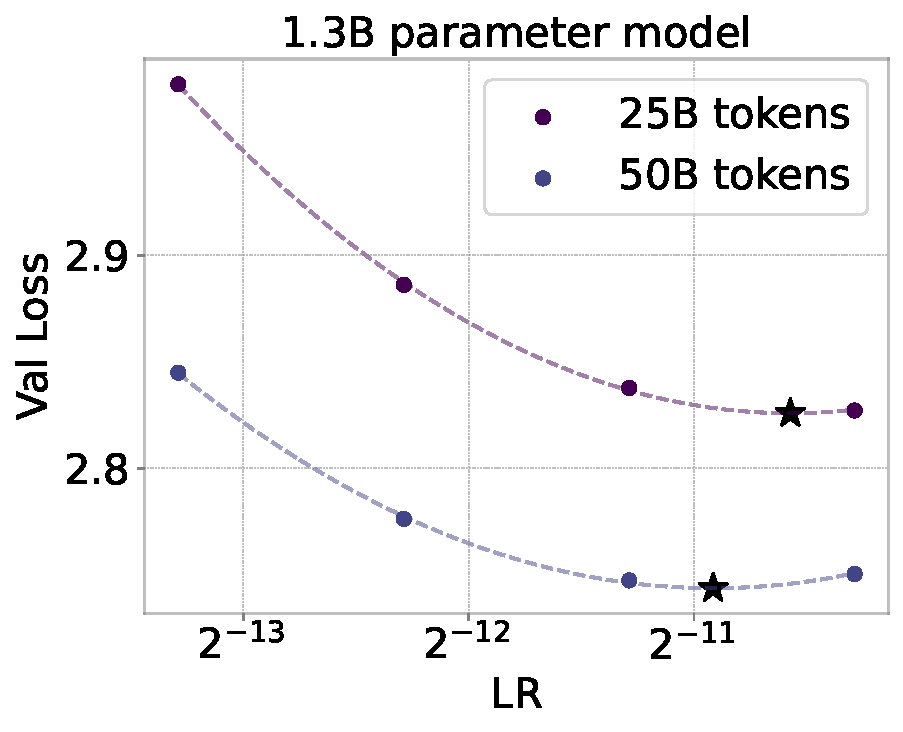
\includegraphics[width=0.5\textwidth]{images/bs_1b.pdf}
\caption{Learning rate and validation loss for different token horizons for the 1.3B model from \Cref{table:param} using 1m batch size.}
\label{fig:curves_bs}
\centering
\end{center}
\end{figure}


\begin{figure}[]
\begin{center}
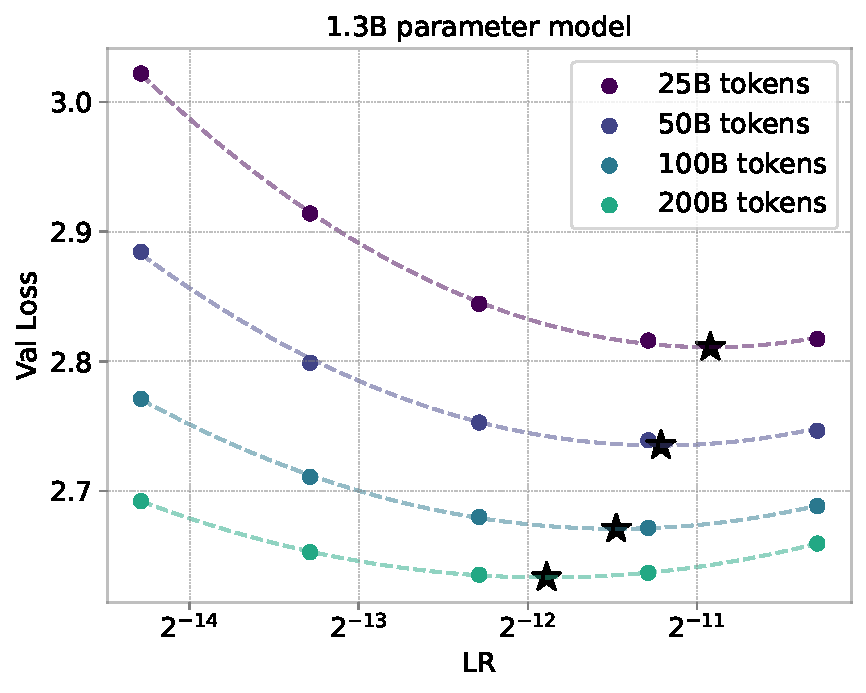
\includegraphics[width=0.6\textwidth]{images/1b.pdf}
\vspace{-0.3cm}
\caption{Learning rate and validation loss for different token horizons for the 1.3B model of \Cref{table:param}. We see that the optimal LR decreases as the token horizon increases.}
\label{fig:1bmodel_firstimg}
\centering
\end{center}
\end{figure}


\begin{figure}[]
\begin{center}
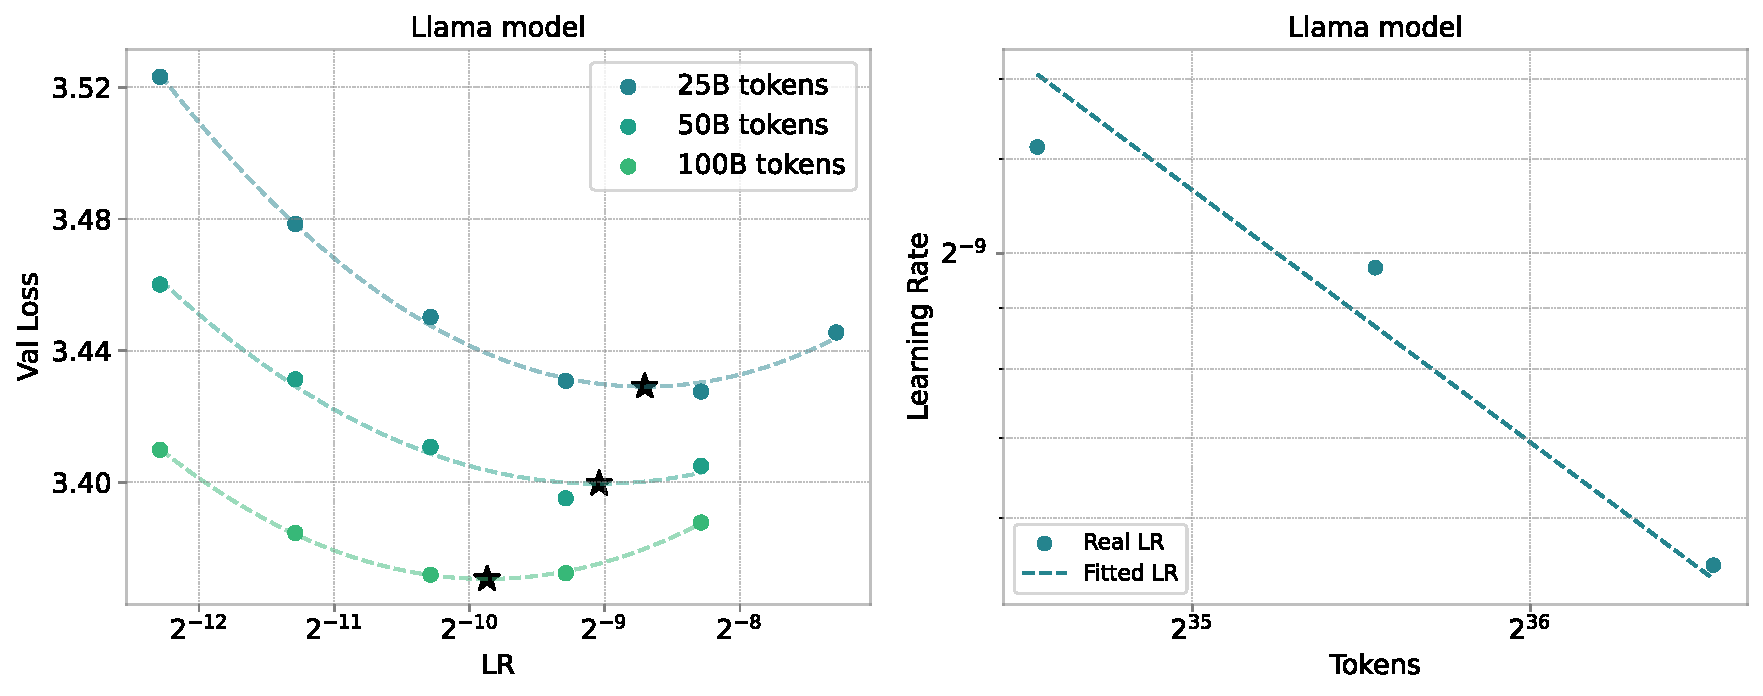
\includegraphics[width=\textwidth]{images/reb/gated-both.pdf}
\vspace{-0.3cm}
\caption{\rebuttal{Experiments on the 50m model using the Llama-1 architecture (RMSnorm, Rope embeddings, and so on) of \cite{llama1}. Similar to the GPT-3 architecture, we see that optimal LR decreases with the token horizon. On the right we plot the scaling law, using the same $\beta$ as the GPT-3 model. We see an excellent fit, demonstrating that the $\beta$ transfers well across model architectures.}}
\label{fig:gated_both}
\centering
\end{center}
\end{figure}



\begin{figure}[]
\centering
\begin{minipage}[b]{0.45\linewidth}
    \centering
    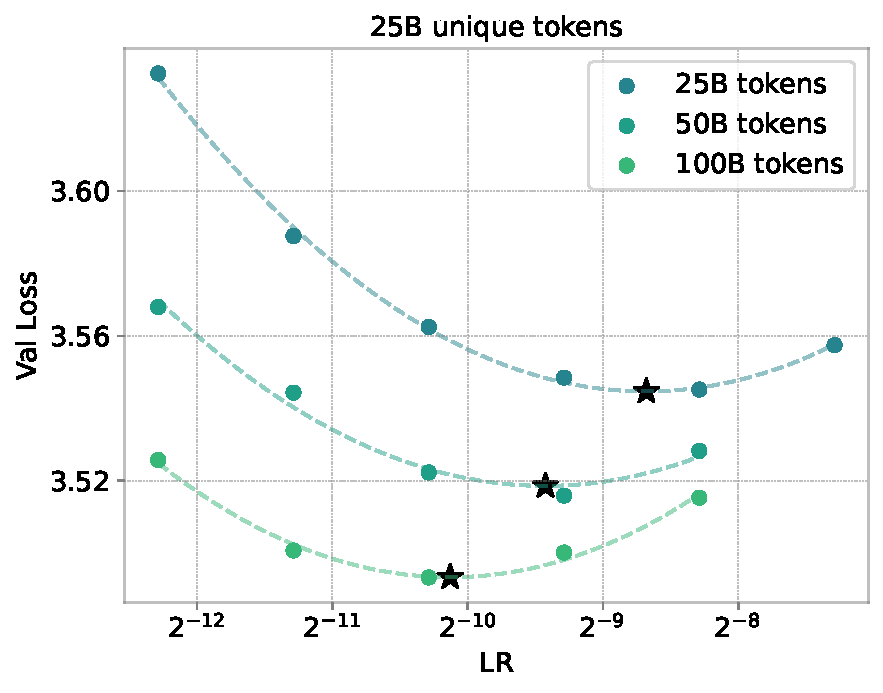
\includegraphics[width=\linewidth]{images/reb/post-rebuttal/fixed_100b.pdf}
\end{minipage}
\begin{minipage}[b]{0.45\linewidth}
    \centering
    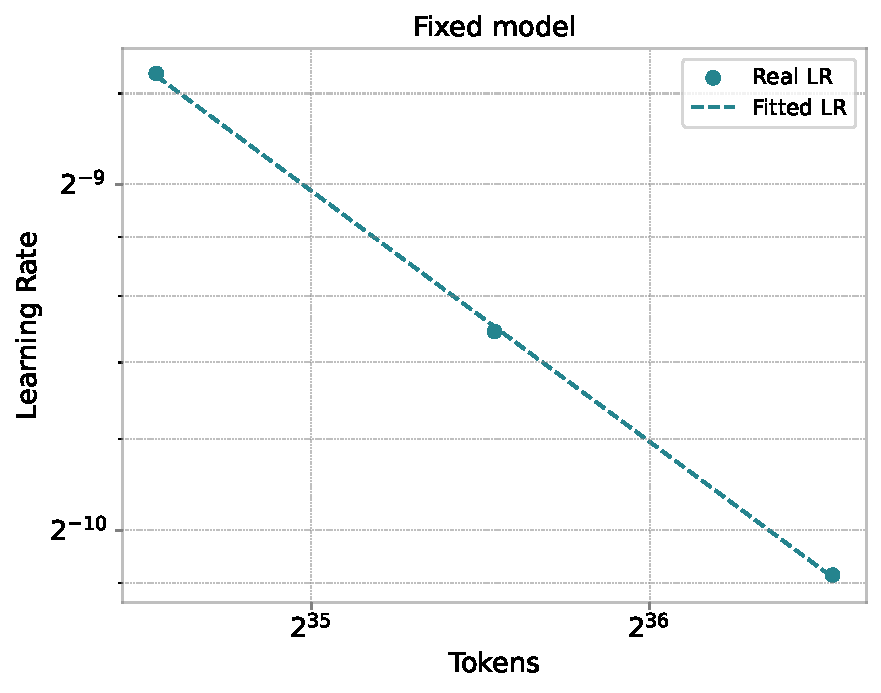
\includegraphics[width=\linewidth]{images/reb/post-rebuttal/fit_fixed_100b.pdf}
\end{minipage}
\vspace{-0.3cm}
\caption{We sample a set of 25B unique tokens, and ablate LR when the training horizon is 25B, 50B and 100B tokens. This corresponds to one, two, or four epochs over the data. We use the 50m model. (Left) The optimal LR decreases when we increase the total token horizon, thus the total number of unique tokens seen does not solely determine the optimal LR. (Right) The slope between the optima in this setting fits the scaling curve from training only only unique tokens. This suggests that it is the token horizon rather than the number of unique tokens which determines the scaling.}
\label{fig:fixed_tokens}
\centering
\end{figure}



\begin{figure}[]
    \centering
    \begin{minipage}[b]{0.45\linewidth}
        \centering
        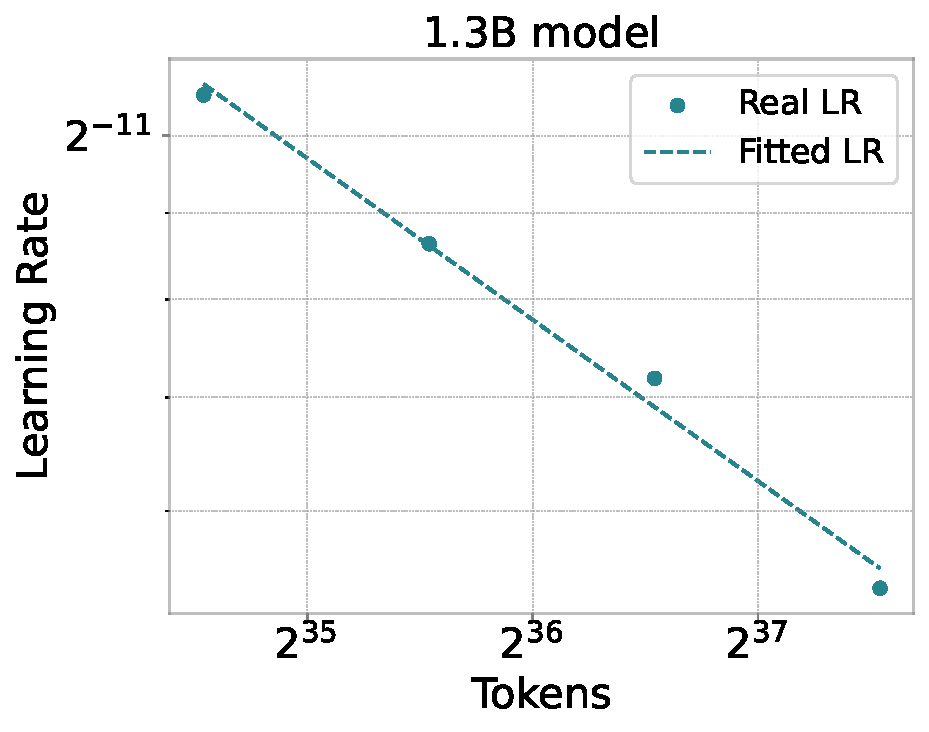
\includegraphics[width=\linewidth]{images/fit_1b.pdf}
    \end{minipage}
    \begin{minipage}[b]{0.45\linewidth}
        \centering
        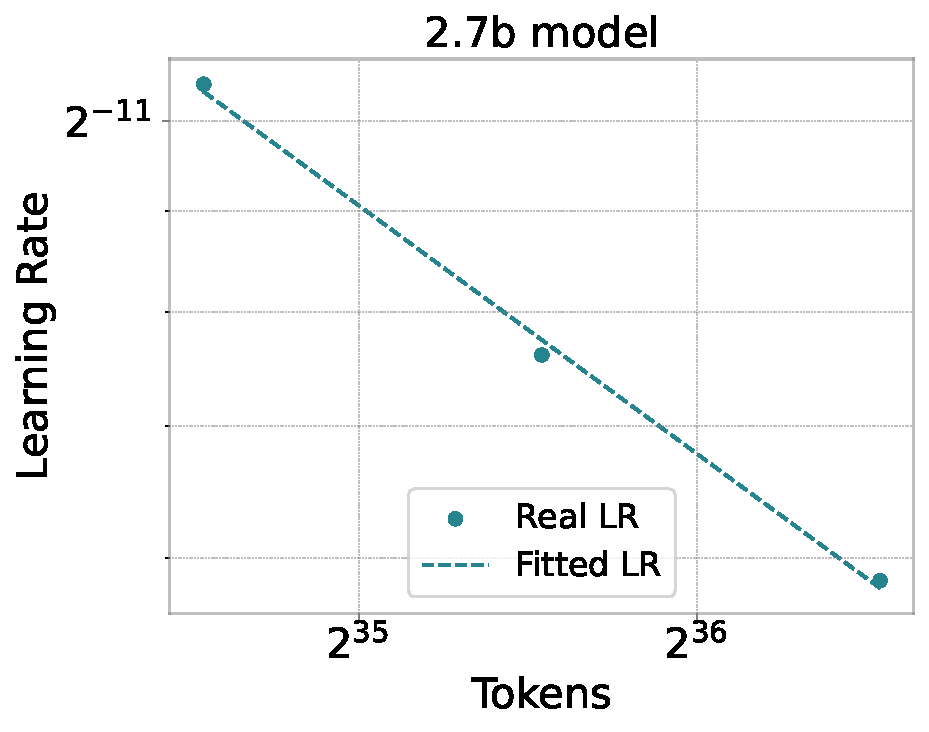
\includegraphics[width=\linewidth]{images/fit_2b.pdf}
    \end{minipage}
    \vspace{-0.3cm}
    \caption{Optimal LR as a function of token horizon for the 1.3B and 2.7B models. A straight-line provides a good fit, indicating that the power-law of \Cref{eq:powerlaw} works well. See \Cref{sec:scaling_laws} for further details.}
    \label{fig:single_fit_1b2b}
    \vspace{-0.3cm}
\end{figure}





\begin{table}[]
    \begin{center}
\begin{tabular}{lrrrr}
\toprule
seed &  $L($\scinot{1.5}{-4}$)$ &  $L($\scinot{3}{-4}$)$ & $L($\scinot{6}{-4}$)$ &   $\argmin L$  \\
\midrule
1    &  2.940372 &  2.919948 &  2.913585 &  \scinot{5.81}{-4}  \\
2    &  2.941199 &  2.919131 &  2.912387 &  \scinot{5.76}{-4} \\
3    &  2.941648 &  2.920779 &  2.915190 &  \scinot{5.47}{-4} \\
\bottomrule
\end{tabular}
    \end{center}
    \caption{We consider the loss $L$ as a function of the LR. We repeat the experiments of \Cref{sec:initial_abl} with a 100B token horizon, a 350m model, and multiple seeds. With different seeds, we see slightly different final losses, and slightly different estimates of the optimal LR.}
    \label{table:seed_stds}
\end{table}

\begin{figure}[]
\begin{center}
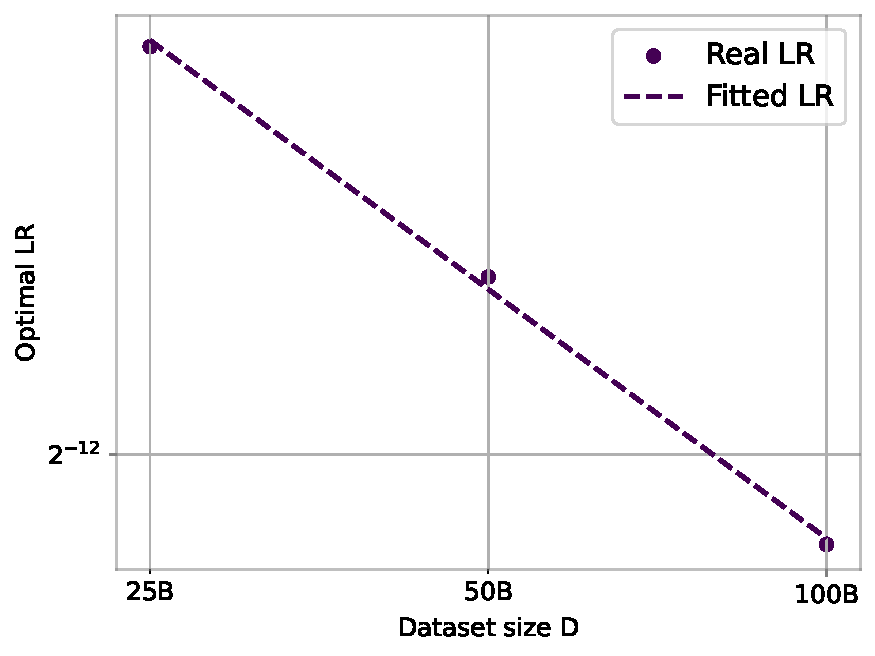
\includegraphics[width=0.6\textwidth]{images/opt_lr_d_n7b.pdf}
\vspace{-0.3cm}
\caption{Optimal LR vs token horizon for a $7B$ LLama-1 model using batch size of $4M$. \johan{needs longer caption which is self-contained}}
\label{fig:7b}
\centering
\end{center}
\end{figure}


\begin{figure}[h]
\begin{center}
\vspace{-0.5cm}
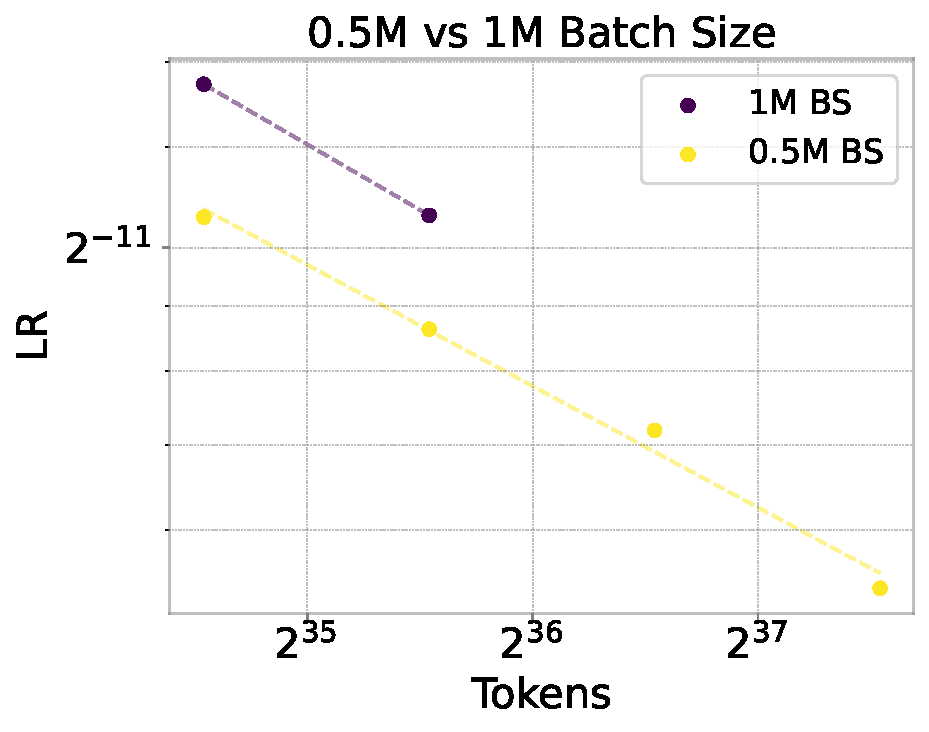
\includegraphics[width=0.5\textwidth]{images/bs_fit.pdf}
\vspace{-0.3cm}
\caption{Optimal LR as a function of token horizon for a 1.3B model using a batch size of 0.5m or 1m tokens. A larger batch size implies that a larger LR is optimal, as expected. The two lines are roughly parallel, suggesting that the dependence on token horizons is the same irrespective of the batch size.}
\label{fig:bs_main}
\centering
\end{center}
\end{figure}


\begin{table}[h]
\begin{center}
\begin{tabular}{ll}
\toprule
Token Horizon & Optimal LR     \\
\midrule
25B    & $\e{3.4}{-4}$\\
50B & $\e{2.8}{-4}$  \\
100B  & $\e{2.3}{-4}$\\
1T (Using Eq. \ref{eq:powerlaw}  & $\e{1.15}{-4}$\\
1T (Using Eq. \ref{eq:scaling_law}) & $\e{1.1}{-4}$\\
\bottomrule
\end{tabular}
\end{center}
\caption{Optimal LR for LLama-1 for different token horizon using the fit in \Cref{fig:7b}. Note that the real Llama-1 used an LR of \scinot{3}{-4} which our results suggest is significantly too large.}
\label{table:7b_fit}
\end{table}



\begin{table}[h]
    \begin{center}
\setlength{\tabcolsep}{4pt}
\begin{tabular}{lllllll}
\toprule
  &   25B &  50B &      100B &      200B &      400B &      800B \\\midrule
Optimal LR &  \scinot{1.34}{-3} & \scinot{1.02}{-3} & \scinot{6.60}{-4} & \scinot{4.12}{-4} & \scinot{2.51}{-4} & \scinot{1.98}{-4} \\         Predicted LR   &      &               &               & \scinot{4.77}{-4} & \scinot{3.35}{-4} & \scinot{2.35}{-4} \\         Ratio   &      &               &               & 0.864 & 0.749 & 0.843 \\\bottomrule
\end{tabular}
    \end{center}
    \caption{Simulated hyperparameter transfer across token horizons for a 125m model. The setup follows \Cref{table:simulated_transfer_second}.}
    \label{table:simulated_transfer_second}
\end{table}

\begin{table}[h]
    \begin{center}
\begin{tabular}{lll}
\toprule
& $R^2$ & $\beta$ \\
\midrule
$\mu$ & 0.961 & 0.384 \\
$\sigma$ & \scinot{8.85}{-3} &  \scinot{7.78}{-3} \\
$\sigma/\mu$ & \scinot{9.21}{-3} &  \scinot{2.03}{-2} \\
\bottomrule
\end{tabular}
\end{center}
\caption{We show the mean $\mu$, standard deviation $\sigma$ and relative deviation $\sigma/|\mu|$ estimated via bootstrapping for two quantities : the $R^2$ and $\beta$ in \Cref{sec:uncertainty}. The relative deviation of $\beta$ is roughly 10\%, demonstrating that the uncertainty is reasonably small in our scaling laws.}
\label{table:bootstrap_stds_appendix}
\end{table}



\newpage
\FloatBarrier
\section{Derivation}
\label{appendix:derivation}

In section \ref{sec:scaling_laws} we saw empirically that for a given $N$ and constants $B, \beta$ that may be dependent on $N$,
\begin{equation}\label{eq:lrd}
    \optlr(N,D) = B(N) D^{-\beta(N)}
\end{equation}
As seen in \Cref{fig:opt_lr_n_d}, we observe a linear relationship between $\log N$ and $\optlr$ for any given $D$. This suggests the relationship:
\begin{equation}\label{eq:lrn}
    \optlr(N,D) = A(D) N^{-\alpha(D)}
\end{equation}
The constants $A, \alpha$ may depend on $D$. 
The key question that arises is how the general notion of model size $N$ can be incorporated into the joint scaling law. Moreover, the scaling law formula from Eq. \ref{eq:lrn} for constant $D$ has to be representable by Eq. \ref{eq:lrd}. It is anticipated to align with the latter, consisting of distinct power laws, each with specific parameters for different $N$ and $D$ values.
Consequently, the objective is to identify a function that fulfills these criteria

\begin{equation}\label{eq:match}
    \optlr(N,D)=B(N) D^{-\beta(N)}=A(D) N^{-\alpha(D)}
\end{equation}


\textbf{Dataset size $D$ for different Model Size $N$.} As seen in \Cref{fig:opt_lr_d_n}, since the lines are parallel for any given $N$, the slope $\beta$ (Eq. \ref{eq:lrd}) is independent of the model size $N$. Therefore we can assume that $\beta(N)=\beta$.

\textbf{Model size $N$ for different Dataset size $D$.} As seen in \Cref{fig:opt_lr_n_d}, since the lines are parallel for any given $D$, the slope $\alpha$ (Eq. \ref{eq:lrn}) is independent of the dataset size $D$. Therefore we can assume that $\alpha(D)=\alpha$ is constant.

Using the fact that $\alpha,\beta$ are constant and multiplying Eq. $\ref{eq:match}$ by $N^{\alpha} D^{\beta}$:
\begin{equation}\label{eq:match_const}
    B(N) N^{\alpha} =A(D) D^{\beta}
\end{equation}
The LHS of Eq. \ref{eq:match_const} only depends on $N$, whereas the RHS only depends on $D$ so they should both equal some constant, $C$ (this step relies on our proof above that $\alpha,\beta$ are independent of $N,D$), resulting in the functional forms of $A(D),B(N)$
\begin{equation}\label{eq:AB}
   A(D) = CD^{-\beta}, B(N)=CN^{-\alpha}
\end{equation}
Plugging the functional forms of $B(N)$ we finally get the final functional form for the joint scaling law as in Eq. \ref{eq:scaling_law}.

